\chapter{Choix et présentation du commanditaire}

\section{Choix du commanditaire}
Le 3 juillet 2026, lors de la kermesse à l'école Rancher de Nice, ou sont scolarisés mes enfants, j'ai échangé avec la directrice de l'établissement Mme Hélène Fouassier au sujet d'une éventuelle intervention de sécurité routière auprès d'élèves de CM2. Un accord de principe a été évoqué pour l'année scolaire 2026--2027 le même jour. J'ai également pris contact avec un responsable d'une entreprise de sécurité présente lors de l'événement ; cette piste n'a pas donné de suite favorable.

Ma collègue Manane SADIK m’a parlé de l’AFPA de Nice, après avoir obtenu cette information par l’intermédiaire d’une de ses connaissances. Cette piste nous a intéressés, car elle nous permettait de nous adresser à un public adulte confronté à des déplacements liés à la formation et à la future activité professionnelle. Nous avons donc choisi d’explorer cette possibilité afin de travailler sur des situations concrètes de risque routier. Ce choix ne remet pas en cause l’intérêt d’une sensibilisation auprès des enfants, mais il correspondait davantage à notre volonté de travailler sur des comportements et des décisions observables dans un contexte professionnel.

L'AFPA de Nice nous a paru pertinente en raison de la diversité de ses formations et de la possibilité d'aborder les trajets domicile--formation, mais aussi les futurs déplacements entre entreprise, fournisseurs, clients et chantiers. Ce dernier contexte constituait d'abord une \emph{hypothèse de pertinence}, à préciser avec le commanditaire et les stagiaires.

\section{Premier courriel de contact}
Le 3 septembre 2026, nous nous sommes rendus à l'AFPA de Nice en fin de journée. N'ayant pas pu rencontrer directement les responsables, nous avons contacté l'accueil par téléphone pour présenter notre proposition et demander qu'elle soit transmise à la direction.

Le 9 septembre 2026 à 15\,h\,33, nous avons adressé à Mme Muriel LIÉGEOIS un courriel intitulé « \textbf{Proposition d'une action gratuite de sensibilisation à la sécurité routière} ». Nous y présentions le cadre du TP ECSR, la gratuité de l'intervention et une durée envisagée d'environ deux heures.

Nous avons surtout souligné que nous ne souhaitions \textbf{pas imposer un thème} : notre intention était de recueillir les attentes de l'AFPA, d'identifier les éventuelles problématiques et de construire une réponse adaptée au public. Le courriel proposait des pistes ouvertes (fatigue, téléphone, vitesse, alcool, stupéfiants, partage de la route, risques professionnels ou éco-conduite), sans les présenter comme des problèmes établis au sein du centre.

Cette prise de contact poursuivait un double objectif : proposer une action utile aux participants et exercer, dans un cadre réel, les compétences attendues d'un futur enseignant de la conduite.

\section{Entretien téléphonique}
Le 10 septembre 2026 à 11\,h\,23, Mme LIÉGEOIS a répondu favorablement à notre proposition et nous a invités à l'appeler pour en discuter. J'ai donné suite à cette invitation par téléphone. Cet échange a ouvert la phase de clarification du besoin et confirmé l'intérêt d'un questionnaire destiné au commanditaire.

Le 11 septembre, j'ai annoncé l'envoi de ce questionnaire mais omis la pièce jointe. Mme LIÉGEOIS l'a signalé le même jour. Le 23 septembre à 15\,h\,59, j'ai transmis le document avec des excuses. Cette correction fait partie du suivi administratif du projet ; elle rappelle l'importance de contrôler les pièces jointes avant l'envoi d'un document de travail.

\section{Présentation du commanditaire}
L'AFPA est un organisme de formation professionnelle d'adultes. Dans notre projet, l'interlocutrice du commanditaire est Mme Muriel LIÉGEOIS, responsable de formation au centre AFPA Nice/Cannes, situé dans les Alpes-Maritimes.


Le 19 novembre 2026, Mme LIÉGEOIS nous a transmis un organigramme anonymisé du centre AFPA de Nice. Ce document montre une organisation structurée autour d'une direction de centre, de responsables de formation et de fonctions supports. Pour notre action, il confirme que Mme LIÉGEOIS occupe une position d'interface entre les stagiaires, l'équipe pédagogique et l'organisation du site. Cette place dans l'organigramme éclaire son rôle dans notre projet : accueillir la demande, faciliter la coordination de l'action et orienter les échanges vers les interlocuteurs compétents lorsque cela est nécessaire.

\begin{figure}[H]
  \centering
  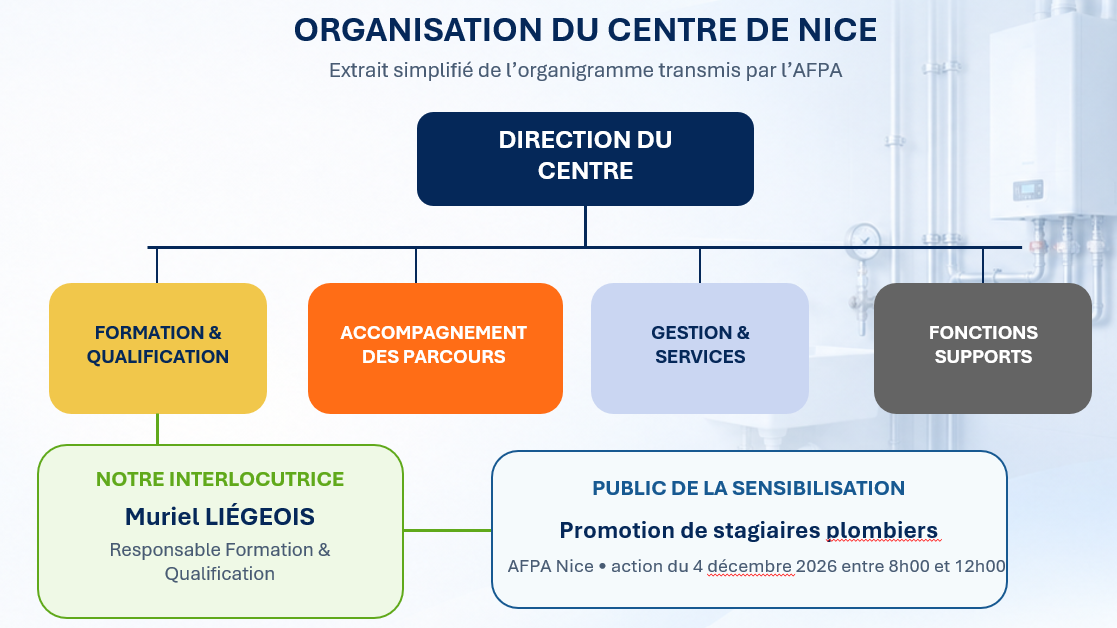
\includegraphics[width=0.72\textwidth,keepaspectratio]{images/organisation_afpa_nice_simplifiee.png}
  \caption{Organisation simplifiée du centre AFPA de Nice, à partir de l'organigramme transmis par le commanditaire.}
  \label{fig:organisation-afpa-nice}
\end{figure}

\section{Entretien avec le commanditaire}
Le 28 septembre, Mme LIÉGEOIS nous a retourné son questionnaire de recueil des besoins et a proposé une date d'intervention. Afin de dépasser la seule lecture du formulaire, j'ai sollicité le même jour un rendez-vous pour préciser le profil des participants et les objectifs attendus. Mme LIÉGEOIS a confirmé un entretien le \textbf{jeudi 1\textsuperscript{er} octobre 2026 à 15\,h}, et nous a adressé une invitation Outlook.

Au cours de cet échange, nous avons réexaminé le public et le format envisagés. Une première estimation d'environ quarante participants a été jugée peu compatible avec une animation participative. Le projet a été recentré sur un groupe d'environ dix à quinze stagiaires, appartenant à une promotion de plomberie et âgés approximativement de dix-huit à trente ans selon les informations fournies. Le statut individuel de conducteur et les habitudes de déplacement restaient à vérifier.

La date finalement proposée par le commanditaire est le \textbf{4 décembre 2026 entre 8h00 et 12h00}. Dans son message du 28 septembre, Mme LIÉGEOIS avait d'abord écrit « 4/11 » puis a explicitement corrigé cette erreur en précisant « 04/12 ». La correction est retenue dans notre chronologie.

